\chapter{توصیف معماری سیستم}
\noindent
\textbf{
	\textit{
		تشریح اینترفیس‌های سیستم، کلاک‌ها و نحوهٔ راه‌اندازی سیستم، دیاگرام بلوکی سخت‌افزار، ساختار درختی سیستم و توصیف ماژول‌های سخت‌افزار 
	}
}
\pagebreak

\section{ اینترفیس‌های سیستم}
در ابتدا به صورت خلاصه اینترفیس‌های سیستم سخت‌افزاری الگوریتم Skein بیان می‌شود، اینترفیس یک سیستم شامل ورودی‌ها و خروجی‌ها و مشخصات ایشان است. 
\subsection{ورودی‌ها}
ورودی‌ها کد verilog الگوریتم Skein به شرح زیر اند.
\begin{itemize}
	\item
	      \textbf{clk}\\
	      ورودی کلاک سیستم است که با آن سیستم کار خود را به صورت ترتیبی 
	      \footnote{\lr{Sequential}}
	      انجام می‌دهد، فرکانس کلاک با توجه به نحوهٔ پیاده‌سازی سخت‌افزاری و نتایج حاصل از سنتز تعیین می‌شود. در Testbench داده شده کلاک هر ۱۰ نانوثانیه تغییر می‌کند.
	\item
	      \textbf{\lr{midstate}}\\
	      ورودی ۵۱۲ بیتی برای الگوریتم
	      \lr{Skein-512}
	      است که حالت میانی در هش را معلوم می‌کند.
	\item
	      \textbf{nonce}\\
	      nonce مقداری دلخواه است که برای به حداکثر رساندن تصادفی  و غیرقابل شکستن بودن هش 
	      در محاسبه هش استفاده می‌شود، این مقدار می‌تواند عددی دلخواه باشد. در الگوریتم 
	      \lr{Skein-512}
	      اندازهٔ این ورودی ۳۲ بیت به اندازه طول عدد در Integer گرفته شده است.
	\item
	      \textbf{data}\\
	      ورودی اصلی‌ست که باید هش آن محاسبه شود، در کد verilog داده شده اندازه این ورودی ۹۶ بیت در نظر گرفته شده است. 
\end{itemize}

\subsection{خروجی}
تنها خروجی سیستم مقدار هش در output است که ۵۱۲ بیت طول دارد.
(الگوریتم مورد بحث 
\lr{Skein-512}
است)

\section{کلاک‌ها و نحوهٔ راه‌اندازی سیستم}
این سیستم فقط از یک کلاک استفاده می‌کند و برای راه‌اندازی سیستم انجام کارهای زیر ضروری‌ست.
\begin{enumerate}
	\item
	      وصل کردن کلاک با فرکانس مناسب به سیستم
	\item
	      اعمال ریست‌ کلی بر سیستم
	      \footnote{\lr{Global Reset}}
	\item 
	      تعیین ورودی‌های اولیه
	      \begin{itemize}
	      \item
				\textit{ ورودی‌های سیستم در ادامه به طور کامل تشریح شده‌اند، هیچ یک از ورودی‌ها نسبت به دیگری تقدم 				زمانی هنگام assignment ندارد.}
	      \end{itemize}
	
	\item 
	      راه‌اندازی سیستم 
\end{enumerate}


\section{دیاگرام بلوکی سخت‌افزار}
دیاگرام بلوکی کلی سخت‌افزار در شکل 
\ref{block_diagram}
آمده است. 

\begin{figure}[H]
	\centering
	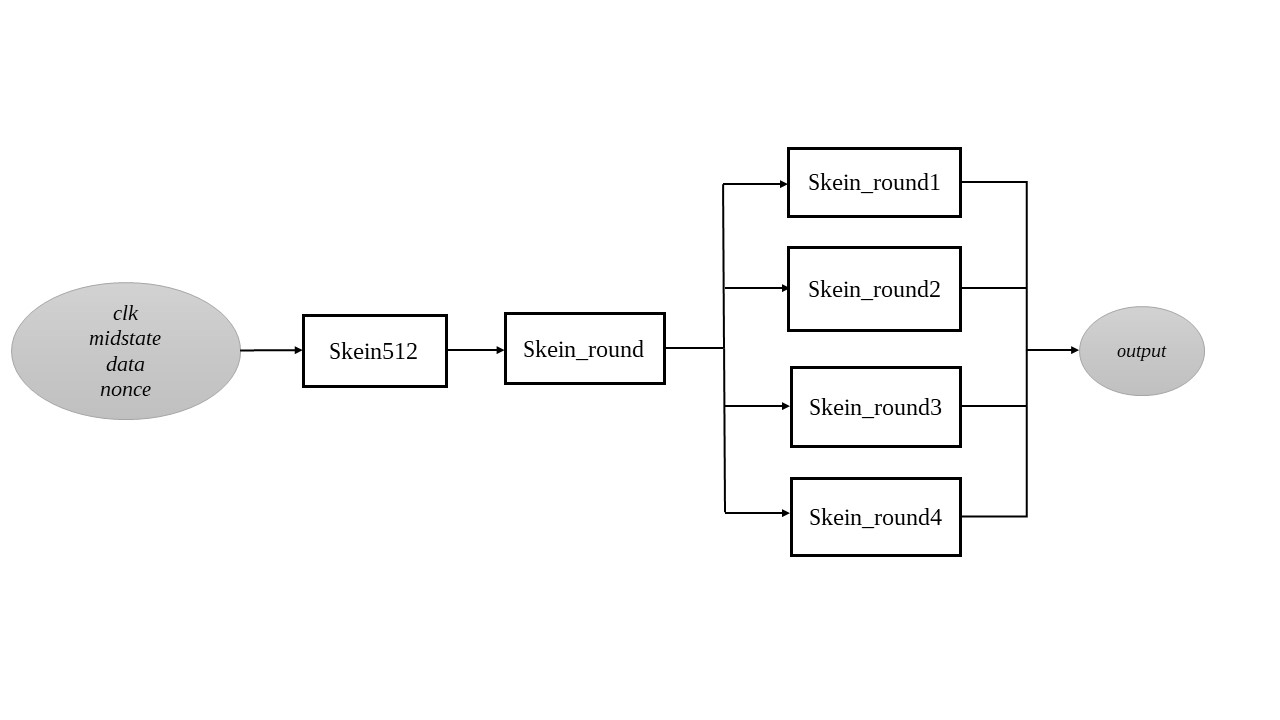
\includegraphics[width = \textwidth]{figs/DescriptionOfSystem/block_diagram.jpg}
	\caption{دیاگرام بلوکی سخت‌افزار}
	\label{block_diagram}
\end{figure}
\begin{figure}[H]
\centering
\begin{subfigure}{.5\textwidth}
  \centering
  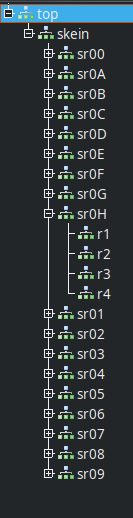
\includegraphics[width=0.5\linewidth]{figs/DescriptionOfSystem/hierarchial_design.png}
  \caption{ساختار ماژول‌ها هنگام شبیه‌سازی}
  \label{module_diagram}
\end{subfigure}%
\begin{subfigure}{.5\textwidth}
  \centering
  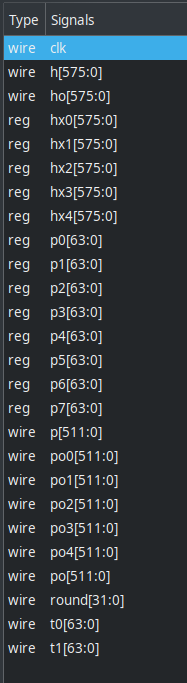
\includegraphics[width=0.5\linewidth]{figs/DescriptionOfSystem/wires_regs.png}
  \caption{ساختار سیگنال‌ها هنگام شبیه‌سازی}
  \label{wire_diagram}
\end{subfigure}
\caption{ساختار درختی سیستم}
\label{hierarchial_design}
\end{figure}

\pagebreak
\section{توصیف ماژول‌های سخت‌افزار}
\subsection{\lr{Skein-512}}
\subsubsection{اطلاعات کلی}
\lr{
\begin{table}[H]
\centering
\begin{tabular}{@{}ll@{}}
\toprule
\multicolumn{2}{l}{skein512}                                           \\ \midrule
$clk, {[}511:0{]} midstate, {[}95:0{]} data, {[}31:0{]} nonce$ & inputs  \\
${[}511:0{]} hash $                                            & outputs \\ \bottomrule
\end{tabular}%
\rl{
\caption{اطلاعات کلی ماژول \lr{skein512}}}
\label{table_skein512}
\end{table}}
درخطوط اولیه تعداد reg و wire تعریف شده است.
دو reg به نام های $ phase\_d$ و $phase\_q $ تعریف شده اند که یک‌بیتی اند و مقدار صفر به آنها داده شده است.\\
دو assignment یک‌خطی دیده می‌شود.

\begin{enumerate}
	\item در reg 32 بیتی با نام $nonce\_le$ که در خطوط بالاتر تعریف شده است مقادیر $nonce$ (که ورودی 32 بیتی ماژول هستند) به صورت 8 بیت – 8 بیت و به صورت برعکس ذخیره می‌شوند. یعنی به طور مثال 8 بیت کم ارزش\  $nonce$در 8 بیت پرارزش $nonce\_le$ ذخیره شده اند.
	      
	\item در reg 32 بیتی با نام $nonce2\_le$ که در خطوط بالاتر تعریف شده است مقادیر $nonce2$ (که برعکس $nonce$، ورودی ماژول نیست و خود در خطوط بالاتر به صورت یک reg 32 بیتی تعریف شده است و در واقع در حال حاضر مقداری را به خود اختصاص نداده است) به صورت 8 بیت – 8 بیت و به صورت برعکس ذخیره می‌شوند. یعنی به طور مثال 8 بیت کم ارزش\  $nonce2$ در 8 بیت پرارزش  $nonce2\_le$ ذخیره شده اند. (خط 56)
\end{enumerate}

یک عبارت assign طویل مربوط به hash دیده می‌شود:

\begin{itemize}
	\item
	      در این عبارت بیت‌های رجیستری به نام
	      $h\_q$ 
	      که 512 بیت دارد و در خطوط بالاتر تعریف شده است، به بیت های خروجی hash اساین می‌شود.
	\item
	      64 مجموعه 8بیتی از $h\_q$ به بیت های hash اساین می‌شود که نظم این مقداردهی در زیر توضیح داده می‌شود. در این توضیحات hash را به ترتیب از پرارزش‌ترین ۸بیت شروع به پر کردن می‌کنیم.
	\item
	      پرارزش‌ترین بیت‌های hash با بیت های $463$ تا $456$ پر شده است. (یعنی پرارزش‌ترین بیت hash با بیت $463$ ام $h\_q$ پر شده است و به همین ترتیب)
	\item
	      مجموعه بعدی 8تایی از $464$ تا $471$ هستند که در دومین 8تایی با ارزش hash قرار می‌گیرند.
	\item
	      این روند تا هشتمین 8بیت ارزشمند hash ادامه پیدا می‌کند جایی که در این جایگاه مجموعه $[511:504]$ از $h\_q$ جای می‌گیرد. (تا اینجا نظم داشتیم)
	\item
	      نهمین 8 بیت ارزشمند hash توسط بیت های $[391:384]$ از $h\_q$ پر می‌شوند.
	\item
	      این روند ادامه پیدا می‌کند (یعنی دهمین 8 بیت ارزشمند با $[399:392]$ پر می‌شوند)،
	      تا 16امین 8 بیت ارزشمند hash که با مجموعه $[447:440]$ پر شده‌اند.
	\item
	      17امین 8 بیت ارزشمند با مجموعه $[327:320]$ پر می‌شود.
	\item
	      این روند مانند قبل به صورت صعودی ادامه پیدا خواهد کرد تا به 25امین مجموعهٔ 8بیتی برسیم.
	      
\end{itemize}

\textit{\textbf{درواقع هر 8 بار که مجموعه بیت‌های 8بیتی را assign می‌کنیم، یک بی‌نظمی داریم.
}}
\begin{itemize}
	\item
	      25امین 8بیتی hash با بیت‌های $[263:256]$ پر می‌شود.
	\item
	      دوباره روند سابق و صعودی را داریم تا به 33امین assignment برسیم.
	\item
	      33امین 8بیتی hash با بیت‌های $[199:192]$
	      
\end{itemize}

\textit{\textbf{هر بار بی‌نظمی داریم بازه جدید بعد از بی نظمی 120 واحد کمتر از بازه قبلی خواهد بود مثلا 32امین 8بیت پرارزش hash با بیت های $[319:312] $پر شده‌اند که 120 واحد از بازه ای که برای 33امین 8 بیت ارزشمند hash اختصاص داده می‌شود بیشتر است. (در بالا 33امین نوشته شده است)}}

\begin{itemize}
	\item
	       8 مجموعه که به صورت صعودی پیش برویم به 40امین 8بیت می‌رسیم که طبق نظم با بیت های $[255:248]$ پر شده است و 41امین 8 بیتی با بازه $[135:128]$ پر شده است.
	\item
	       8 مجموعه که به صورت صعودی پیش برویم به 48امین 8بیت می‌رسیم که طبق نظم با بیت های $[191:184]$ پر شده است و 49امین 8 بیتی با بازه $[71:64]$ پر شده است.
	\item
	       8 مجموعه که به صورت صعودی پیش برویم به 56امین 8بیت می‌رسیم که طبق نظم با بیت های $[127:120]$ پر شده است و 57امین 8 بیتی با بازه $[7:0]$ پر شده است.
	\item
	      از 57امین مجموعه 8 تایی با ارزش hash تا آخرین مجموعه باارزش hash (64امین) نیز به صورت صعودی و طبق نظم پیش می‌رود. (خط 121)
	      
\end{itemize}

بعد از خطوط 
assignment،
 ۱۸ instance از ماژول skein\_round گرفته شده است.
این instance ها را از 
$00$
تا
$0H$
نام‌گذاری کردیم (نام‌گذاری در مبنای بالاتر از 10 شده است)

\subsubsection{
	ورودی skein\_round ها
}
\begin{itemize}
	\item
	      \textbf{کلاک}
	      که همه به کلاک سیستم متصل اند.
	\item
	      \textbf{Round}
	      رجیستر 32بیتی که به ترتیب ورودی 0 تا 17 به هر اینستنس داده شده است.
	\item
	      \textbf{$\textbf{p}$} 
	      رجیستر 512بیتی – که به اینستنس شماره $01$ تا $0H$ به ترتیب $p01$ تا $p0H$ وصل شده است. به اینستنس شماره $00$ هم $p00\_q$ وصل شده است.
	\item
	      \textbf{$\textbf{H}$}
	      رجیستر 576بیتی – که به اینستنس شماره $01$ تا $0H $به ترتیب $h01$ تا $h0H$ وصل شده است. به اینستنس شماره $00$ هم $h00\_q$ وصل شده است.
	\item
	      \textbf{$\textbf{T0}$}
	      رجیستر 64بیتی –   که به اینستنس شماره $00$ تا $0H$ به ترتیب این دنباله سه‌تایی وصل شده است:
	      $t0\_q, t1\_q, t2\_q$
	      این دنباله سه‌جمله‌ای به ترتیب تکرار می‌شود.
	\item
	      \textbf{$\textbf{T1}$}
	      رجیستر 64بیتی – دقیقا مثل $T0$ با این تفاوت که دنباله سه‌تایی $ t1\_q، t2\_q, t0\_q $ به این شکل است.
	\item
	      \textbf{$\textbf{P0}$}
	      رجیستر 512بیتی- که اینستنس شماره $00$ تا $0H$به ترتیب $o00$ تا $o0H$ وصل شده است. 
	\item
	      \textbf{$\textbf{H0}$}
	      رجیستر 576بیتی- که اینستنس شماره $00$ تا $0H $به ترتیب $ho00 $تا $ho0H$ وصل شده است. خط(141)
	      
\end{itemize}
\textit{\textbf{
	در ادامه یک always بلاک داریم که حساس به تغییرات همه چیز است. (خط 143)
	در این بلاک متغیرهایی که در انتهایشان
	\_d
دارند مقداردهی می‌شوند.}}\\
\newline
ابتدا phase\_d مقدار not متغیر phase\_q را به خود اختصاص می‌دهد.
\begin{itemize}
	\item
	      \textbf{اگر phase\_q یک باشد}
	      \begin{itemize}
	      	\item
	      	      مقداردهی به $p00\_d$ (512بیتی): 64 بیت کم‌ارزش ( $[63:0]$) از data در 64 بیت پرارزش $p00\_d$ قرار می‌گیرد. سپس در 32 بیت بعدی $p00\_d$ (از چپ) عینا nonce\_le قرار داده می‌شود. سپس 32 بیت باقی‌مانده از $data ([95:64])$ طبق روند قرار داده می‌شود. باقی بیت‌های این رجیستر هم با صفر پر می‌شوند $(384'd)$ – (خط 148)
	      	\item
	      	      مقداردهی به$ h00\_d$ (576بیتی): در 64 بیت کم‌ارزش این reg مقدار صفر قرار داده میش‌ود و باقی بیت‌ها دقیقا به midstate (ورودی 512 بیتی) متصل می‌شوند.
	      	\item
	      	      مقداردهی به$ t0\_d$ (64 بیتی) : $h0000000000000050$
	      	\item
	      	      مقداردهی به$ t1\_d$ (64 بیتی) : $hb000000000000000$
	      	\item
	      	      مقداردهی به $t2\_d$ (64 بیتی) : $hb000000000000050$
	      	\item
	      	      h\_d هم مقدار h\_q را به خود می‌گیرد.
	      \end{itemize}
	\item
\textbf{	      اگر phase\_q صفر باشد
}	      \begin{itemize}
	      	\item
	      	      مقداردهی به $p00\_d$ (512بیتی): این reg با صفر پر می‌شود.
	      	\item
	      	      مقداردهی به $h00\_d$ (576 بیتی):
	      	      \begin{itemize}
	      	      	\item
	      	      	      بیت‌های $[575:512]$:	
	      	      	      	$data[63:0] \textasciicircum ( oH[511:448] + hH[575:512])$
	      	      	\item
	      	      	      بیت‌های $[511:448]$: 
	      	      	      	\{ $nonce2\_le$ , $data[95:64$ \} \textasciicircum ( $oH[447:384] + hH[511:448]$)
	      	      	\item
	      	      	      بیت‌های $[447:384]$:  $	oH[383:320] + hH[447:384]$
	      	      	\item
	      	      	      بیت‌های $[383:320]$:$	oH[319:256] + hH[383:320]$
	      	      	\item
	      	      	      بیت‌های $[319:256]$:$	oH[255:192] + hH[319:256]$
	      	      	\item
	      	      	      بیت‌های $[255:192]$:
	      	      	      $	oH[191:128] + hH[255:192] + 
	      	      	      64'h0000000000000050$
	      	      	\item
	      	      	      بیت‌های $[191:128]$:	
	      	      	      $oH[127: 64] + hH[191:128] + 64'hb000000000000000$
	      	      	\item
	      	      	      بیت‌های $[127:64]$:
	      	      	  $    	oH[ 63:  0] + hH[127: 64] + 18$
	      	      \end{itemize}
	      	\item
	      	      مقداردهی به$ t0\_d$ (64 بیتی) : $h0000000000000008$
	      	\item
	      	      مقداردهی به $t1\_d$ (64 بیتی) : $hFF00000000000000$
	      	\item
	      	      مقداردهی به $t2\_d$ (64 بیتی) : $hFF00000000000008$
	      	\item
	      	      مقداردهی به $h\_d$ (512 بیتی):
	      	      \begin{itemize}
	      	      	\item
	      	      	      بیت‌های $[511:448]$:
	      	      	      $ 	o0H[511:448] + ho0H[575:512]$
      	      	    \item
	      	      	      بیت‌های $[447:384]$:  
	      	      	      	$o0H[447:384] + ho0H[511:448]$
	      	      	\item
	      	      	      بیت‌های $[383:320]$:
	      	      	      $	o0H[383:320] + ho0H[447:384]$
	      	      	\item
	      	      	      بیت‌های $[319:256]$:
	      	      	      $	o0H[319:256] + ho0H[383:320]$
	      	      	\item
	      	      	      بیت‌های $[255:192]$:
	      	      	      $	o0H[255:192] + ho0H[319:256]$
	      	      	\item
	      	      	      بیت‌های $[191:128]$:	
	      	      	      $o0H[191:128] + ho0H[255:192] + 64'h0000000000000008$
	      	      	\item
	      	      	      بیت‌های $[127:64]$:	
	      	      	      $o0H[127: 64] + ho0H[191:128] + 64'hFF00000000000000$
	      	      	\item
	      	      	      بیت‌های $[63:0]$:	
	      	      	      $	o0H[ 63:  0] + ho0H[127: 64] + 18$
	      	      	 
	      	      \end{itemize}
	      \end{itemize}
\end{itemize}
\textit{
	\textbf{نظم مناسبی دیده می‌شود به این شکل که به ترتیب 64 بیت پرارزش h\_d با مجموع 64 بیت پرارزش $o0H$ و 64 بیت پرارزش $ho0H$ پر می‌شود. به جز 3 مورد آخر که با اعدادی ثابت هم جمع می‌شوند.
}}\\

\textit{\textbf{Always بلاک دوم فقط به لبه مثبت کلاک حساس است. (خط 211)
	(عموما متغیر های \_q مقادیر متناظر \_d را به خود می‌گیرند) }}
\begin{itemize}
	\item
	      $hH$ مقدار $ho0H$ را به خود می‌گیرد.
	\item
	      $oH$ مقدار $o0H$ را به خود می‌گیرد.
	\item
	      $phase\_q$ مقدار $phase\_d$ را به خود می‌گیرد.
	\item
	      $h\_q$ مقدار $h\_d$ را به خود می‌گیرد.
	\item
	      $t0\_q$ مقدار $t0\_d$ را به خود می‌گیرد.
	\item
	      $t1\_q$ مقدار $t1\_d$ را به خود می‌گیرد.
	\item
	      $t2\_q$ مقدار $t2\_d$ را به خود می‌گیرد.
	\item
	      در ادامه مجموعه ای از مقداردهی ها را مربوط به reg های
	       $p0x$
	      و 
	      $h0x$ 
	داریم. (خط 226 تا 261)
	( x منظور از ۱ تا H )
	\item
	      $h0x$ ها: مقدار $ho0y$ را می‌گیرند با این تفاوت که y از x یک واحد کمتر است. (به طور مثال $h01$ مقدار $ho00$ را به خود می‌گیرد)
	\item
	      $p0x$  ها: مقدار $o0y$ را می‌گیرند با این تفاوت که y از x یک واحد کمتر است. (به طور مثال $h01$ مقدار $o00$ را به خود می‌گیرد)
	\item
	      $p00\_q$ مقدار $p00\_d$ را می‌گیرد.
	\item
	      $h00\_q$ مقدار $h00\_d$ را می‌گیرد.
	\item
	      $nonce2$ هم که در ابتدای فایل مقداری مجهول داشت اینجا مقدار $nonce$ (ورودی)  منهای 
	      $32’d54$
	       را می‌گیرد.
\end{itemize}


\subsection{skein\_round}
در خط 124 از فایل وریلاگ، 18 اینستنس از ماژول skein\_round گرفته شده است.
\subsubsection{اطلاعات کلی}
\lr{
\begin{table}[H]
\centering
\begin{tabular}{@{}ll@{}}
\toprule
\multicolumn{2}{l}{skein\_round}                                                            \\ \midrule
$clk, {[}31:0{]} round, {[}511:0{]} p, {[}575:0{]} h, {[}63:0{]} t0, {[}63:0{]} t1 $& inputs  \\
${[}511:0{]} p0, {[}575:0{]} h0 $                                                   & outputs \\ \bottomrule
\end{tabular}%
\rl{
\caption{اطلاعات کلی ماژول \lr{skein\_round}}}
\label{table_skein_round}
\end{table}}
\begin{itemize}
\item
در این ماژول چهار ماژول دیگر زیر ایجاد شده اند. 
\begin{itemize}
\item
\lr{skein\_round\_1}
\item
\lr{skein\_round\_2}
\item
\lr{skein\_round\_3}
\item
\lr{skein\_round\_4}
\end{itemize}
\item
در این ماژول یک 
\lr{always block}
و تعدادی 
\lr{assignment}
وجود دارد.
\item
دو مجموعه reg تعریف شده:
\begin{itemize}
\item
64بیتی: $p0, p1, p2, p3, p4, p5, p6, p7$
\item
576بیتی: $hx0, hx1, hx2, hx3, hx4$
\end{itemize}
\item
یک مجموعه wire تعریف شده:
\begin{itemize}
\item
512بیتی: $po0, po1, po2, po3, po4$
\end{itemize}
\item
3 عدد assignment داریم:
\begin{itemize}
\item
 $ho$ (یکی از خروجی‌ها) از $hx4$ مقدار می‌گیرد. 
 \item
$po$ (دیگر خروجی) از $po4$ مقدار می‌گیرد. 
\item
$Po0$ به ترتیب 8بیت-8بیت (ازپرارزش به کم‌ارزش) از reg های $p0, p1, ..., p7$ مقدار می‌گیرد.
\end{itemize}
\item
از هر 4 ماژول باقی مانده
\lr{(skein\_round\_1,2,3,4)}
 در کد یک اینستنس گرفته شده است. (خط 310)
 
 \begin{itemize}
 \item ورودی کلاک به کلاک سیستم متصل شده است.
ورودی $ even$ ماژول‌ها همگی به  $!round[0]$ متصل اند. (یکی از بیت‌های ورودی)
\item
به عنوان $in$ و $ out $ هم به هر ماژول $po(x)$ و $po(x+1)$ داده می‌شود که $x+1$ شمارهٔ $ round$ ماژول است. به طور مثال به ماژول $skein\_round\_1$ برای ورودی $po0$ و برای خروجی $po1$ داده می‌شود.
 \end{itemize}
\textit{\textbf{ نکته مهم این است که خروجی ماژول 1 ورودی ماژول 2 است و به همین ترتیب تا ماژول ۴.
}}
\item
یک always-block حساس به لبه مثبت کلاک داریم. (خط 315)
\begin{itemize}
\item
ورودی های $h $ و $p $ را به صورت 64بیت – 64بیت جمع می‌زند و در $p0$ تا $p7$ نگه‌داری می‌کند.
\item
به این شکل که جمع پرارزش‌ترین64بیت $h$ و $p$ در $p0$ ریخته می‌شود. (و به همین ترتیب پیش می‌رود)
\item
از $p0$ تا $p4$ کاملا طبق نظم گفته‌شده انجام می‌شود.
\item
در مورد $p5$ علاوه بر دو مجموعهٔ 64بیتی با $t0$ (یکی از ورودی‌ها) هم جمع می‌شود.
\item
در مورد $ p6$ علاوه بر دو مجموعهٔ 64بیتی با$ t1$ (یکی از ورودی‌ها) هم جمع می‌شود.
\item
در مورد $ p7 $ علاوه بر دو مجموعهٔ 64بیتی با $round$ (یکی از ورودی‌ها) هم جمع می‌شود.
\end{itemize}
\item
برای reg های hx (576بیتی) هم یک جابه‌جایی اتفاق میفتد:
\begin{itemize}
\item
به این شکل که $hx4$، مقدار $hx3$ را می‌گیرد.
\item
به این شکل که $hx3$، مقدار$ hx2$ را می‌گیرد.
\item
به این شکل که $hx2$، مقدار $hx1$ را می‌گیرد.
\item
به این شکل که $hx1$، مقدار $hx0$ را می‌گیرد.
\item
برای $Hx0$ اتفاق نسبتا پیچیده‌ای میفتد:
\begin{itemize}
\item
64 بیت کم‌ارزشش با 64 بیت پرارزش $h$ (ورودی) پر می‌شود.
\item
448 بیت پرارزشش  با بیت‌های $[511:64]$ از h پر می‌شود.
\item
64 بیت باقی‌مانده وسط $hx0$ ( $[64:127]$ ) با نتیجهٔ زیر پر می‌شود:  (خط 341)
\begin{code}
((h[575:512] ^ h[511:448]) ^ (h[447:384] ^ h[383:320])) ^ ((h[319:256] ^ h[255:192]) ^  (h[191:128] ^ h[127: 64])) ^ 64'h1BD11BDAA9FC1A22
\end{code}

در واقع در توضیح خط بالا می‌توان گفت $ xor$ تمام مجموعه های 64 بیت‌های ورودی $h $ به جز کم‌ارزش‌ترین مجموعه $( h[64:0] )$ است که در نهایت با یک عدد ثابت 64 بیتی $ xor$ شده است.

\end{itemize}
\end{itemize}
\end{itemize}

\subsection{\lr{skein\_round\_1,2,3,4}}
چهار ماژول باقی‌مانده با نام‌های
\lr{ skein\_round\_1, skein\_round\_2, skein\_round\_3 , skein\_round\_4 }
را به دلیل شباهت ساختاری با هم بررسی می‌کنیم.
\subsubsection{اطلاعات کلی}
\lr{
\begin{table}[H]
\centering
\begin{tabular}{@{}ll@{}}
\toprule
\multicolumn{2}{l}{skein\_round\_1,2,3,4} \\ \midrule
$clk, even, {[}511:0{]} in $   & inputs     \\
${[}511:0{]} out    $          & outputs    \\ \bottomrule
\end{tabular}
\rl{
\caption{ اطلاعات کلی ماژول‌های\lr{ skein\_round\_1,2,3,4}}}
\label{table_skein_round_n}
\end{table}}

\begin{itemize}
\item
در هر 4 ماژول دو مجموعه wire گرفته شده است:
\begin{itemize}
\item
64 بیتی: $p0, p1, p2, p3, p4, p5, p6, p7$
\item
64 بیتی: $ p0x,p1x,p2x,p3x,p4x,p5x,p6x,p7x$
\end{itemize}
\item
مجموعه ای از assignment ها داریم:
\begin{itemize}
\item
$P0$ تا $p7$ به ترتیب به 64 بیت‌های پرارزش تا کم‌ارزش $in$ متصل اند. 
(به کم‌ارزش‌ترین $p7$)
\end{itemize}
\item
Assignment های مربوط به $p0x$ تا $p7x$ برای 4 ماژول متفاوت است در نتیجه جداگانه بررسی می‌کنیم:
\begin{itemize}
\item ماژول ۱\\
$Pkx$ ها با $k$ های زوج مقدار $pk + p(k+1)$ را به خود می‌گیرند. مثلا $p2x = p2 + p3$\\
$P1x$ با توجه به $even$ مقدار می‌گیرد: 
\begin{itemize}
\item
اگر $even$ یک باشد، { $p1[17:0], p1[63:18]$ } (خط شکاف بین بیت 17 و 18)
\item
اگر $even$ صفر باشد، { $p1[24:0], p1[63:25]$ } (خط شکاف بین بیت 24 و 25)
\end{itemize}
   $P3x$ با توجه به $even$ مقدار می‌گیرد: 
 \begin{itemize}
 \item
 اگر $even$ یک باشد، { $p3[27:0], p3[63:28]$ }  (خط شکاف بین بیت 27 و 28)
\item 
اگر $even$ صفر باشد، { $p3[33:0], p3[63:34]$ } (خط شکاف بین بیت 33 و 34)

 \end{itemize}
   $P5x$ با توجه به $even$ مقدار می‌گیرد:
   \begin{itemize}
   \item
   اگر $even$ یک باشد، { $p5[44:0], p5[63:45]$ }  (خط شکاف بین بیت 44 و 45)
   \item
اگر $even$ صفر باشد، { $p5[29:0], p5[63:30]$ } (خط شکاف بین بیت 29 و 30)
\end{itemize}    
   $P7x$ با توجه به $even$ مقدار می‌گیرد: 
   \begin{itemize}
   \item
   اگر $even$ یک باشد، { $p7[26:0], p7[63:27]$ }  (خط شکاف بین بیت 26 و 27)
   \item
اگر $even$ صفر باشد، { $p7[39:0], p7[63:40]$ } (خط شکاف بین بیت 39 و 40)

   \end{itemize}
\item ماژول ۲
\begin{code}
	//module 2 
	assign p0x = p0 + p3
	assign p1x = (even) ? { p1[30:0], p1[63:31] } : { p1[50:0], p1[63:51] }
	assign p2x = p2 + p1
	assign p3x = (even) ? { p3[21:0], p3[63:22] } : { p3[46:0], p3[63:47] }
	assign p4x = p4 + p7
	assign p5x = (even) ? { p5[49:0], p5[63:50] } : { p5[53:0], p5[63:54] }
	assign p6x = p6 + p5
	assign p7x = (even) ? { p7[36:0], p7[63:37] } : { p7[13:0], p7[63:14] }
\end{code}
با توجه به توضیحات در مورد ماژول 1، در ماژول 2 با حفظ کلیات جزئیات تغییر می‌کند.

\item ماژول ۳
\begin{code}
	//module 3
	assign p0x = p0 + p5
	assign p1x = (even) ? { p1[46:0], p1[63:47] } : { p1[38:0], p1[63:39] }
	assign p2x = p2 + p7
	assign p3x = (even) ? { p3[14:0], p3[63:15] } : { p3[34:0], p3[63:35] }
	assign p4x = p4 + p1
	assign p5x = (even) ? { p5[27:0], p5[63:28] } : { p5[24:0], p5[63:25] }
	assign p6x = p6 + p3
	assign p7x = (even) ? { p7[24:0], p7[63:25] } : { p7[20:0], p7[63:21] }
\end{code}
\item ماژول ۴
\begin{code}
	//module 4
	assign p0x = p0 + p7
	assign p1x = (even) ? { p1[19:0], p1[63:20] } : { p1[55:0], p1[63:56] }
	assign p2x = p2 + p5
	assign p3x = (even) ? { p3[ 7:0], p3[63: 8] } : { p3[41:0], p3[63:42] }
	assign p4x = p4 + p3
	assign p5x = (even) ? { p5[ 9:0], p5[63:10] } : { p5[ 7:0], p5[63: 8] }
	assign p6x = p6 + p1
	assign p7x = (even) ? { p7[54:0], p7[63:55] } : { p7[28:0], p7[63:29] }
\end{code}
ماژول های 3 و 4 هم در این مورد مشابهت دارند با توضیحات داده شده در مورد ماژول 1، $pkx$ های با$ k$ زوج مجموع دو $p$ هستند.  اگر $k$ فرد باشد،  $pkx$ برابر همان $pk$ خواهد بود با این تفاوت که با توجه به صفر یا یک بودن $even$ بین یکی از بیت های $pk$ شکاف می‌اندازد و سمت چپ شکاف را در قسمت کم‌ارزش خود و سمت راست شکاف را در قسمت پرارزش پر می‌کند. (در واقع همان rotation که در توصیف الگوریتم بیان شد این‌جا دیده می‌شود).
\end{itemize}
\item
تنها always-block در ماژول (حساس به لبه مثبت کلاک) :\\
در این بلاک خروجی $out$، به صورت مجموعه های 64بیتی مقداردهی می‌شود. $Out$ 512 بیتی است پس 8 بار مقداردهی لازم است. برای هر 4 ماژول مقدارهای نسبت‌داده‌شده به 64بیتی های $out$ را (به ترتیب از پرارزش‌ترین 64بیت تا کم‌ارزش‌ترین آن) داریم :
\begin{itemize}
\item ماژول ۱
\lr{
\begin{table}[H]
\centering
\begin{tabular}{@{}lllllllll@{}}
\toprule
0                        & 1   & 2                        & 3   & 4                        & 5                        & 6   & 7   & Index \\ \midrule
$p7x \textasciicircum p6x$ & $p6x$ & $p5x \textasciicircum p4x$ & $p4x$ & $p3x \textasciicircum p2x$ & $p1x \textasciicircum p0x$ & $p2x$ & $p0x$ & Value \\ \bottomrule
\end{tabular}
\label{table_skein_round_1}
\end{table}}
\item ماژول ۲
\lr{
\begin{table}[H]
\centering
\begin{tabular}{@{}lllllllll@{}}
\toprule
0 & 1 & 2 & 3 & 4 & 5 & 6 & 7 & Index \\ \midrule
$p7x \textasciicircum p4x$ & $p6x$ & $p5x \textasciicircum p6x$ & $p4x$ & $p3x \textasciicircum p0x$ & $p2x$ & $p1x \textasciicircum p2x$ & $p0x$ & Value \\ \bottomrule
\end{tabular}
\label{table_skein_round_2}
\end{table}}
\item ماژول ۳
\lr{
\begin{table}[H]
\centering
\begin{tabular}{@{}lllllllll@{}}
\toprule
0 & 1 & 2 & 3 & 4 & 5 & 6 & 7 & Index \\ \midrule
$p7x \textasciicircum p2x$ & $p6x$ & $p5x \textasciicircum p0x$ & $p4x$ & $p3x \textasciicircum p6x$ & $p2x$ & $p1x \textasciicircum p4x$ & $p0x$ & Value \\ \bottomrule
\end{tabular}
\label{table_skein_round_3}
\end{table}}
\item ماژول ۴
\lr{
\begin{table}[H]
\centering
\begin{tabular}{@{}lllllllll@{}}
\toprule
0 & 1 & 2 & 3 & 4 & 5 & 6 & 7 & Index \\ \midrule
$p7x \textasciicircum p0x$ & $p6x$ & $p5x \textasciicircum p2x$ & $p4x$ & $p3x \textasciicircum p4x$ & $p2x$ & $p1x \textasciicircum p6x$ & $p0x$ & Value \\ \bottomrule
\end{tabular}
\label{table_skein_round_4}
\end{table}}
\end{itemize}
\end{itemize}